\documentclass[a4paper,12pt]{article}
\usepackage[utf8]{inputenc}
\usepackage[T2A]{fontenc}
\usepackage[english,russian]{babel}
\usepackage{graphicx}
\usepackage{lipsum}
\usepackage{float}
\usepackage{trivfloat}
\usepackage[hidelinks]{hyperref}
\usepackage{caption}
\graphicspath{{CSLab4photo/}}
\begin{document}

\section{Цель работы}

Изучить графические возможности \LaTeX.

\section{Задание}

Изучить возможность добавления изображений и ссылок в документ.

\section{Выполнение лабораторной работы}

\subsection{Пакеты и функции для работы с картинками и ссылками}

Для того, чтобы работать с изображениями необходимо использовать пакет \textbf{graphicx}.

В свою очередь в данной работе представлен способ добавления изображения внутрь текста и поэтому введен дополнительный пакет, который создает произвольные абзацы \textbf{lipsum}.

Пакеты \textbf{float} и \textbf{trivfloat} позволяют нам работать с плавающими объектами.

А пакет \textbf{hyperref} с опцией \texttt{hidelinks} делает возможным создание гиперссылок.

При работе с большим количеством изображений, когда обычно они все собираются в одну папку, используется \textbf{graphicspath}, который указывает путь, по которому программа будет искать изображения.

\begin{figure}[h]
\centering
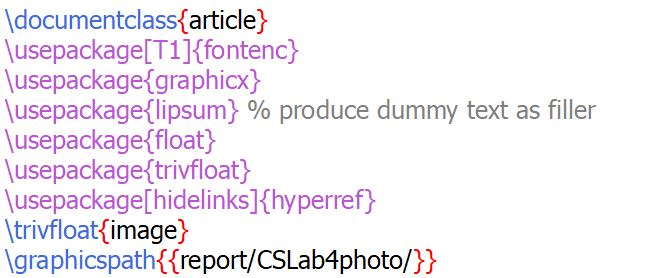
\includegraphics[width=0.5\textwidth]{bibl.JPG}
\caption{Подключение пакетов}
\label{fig:packages}
\end{figure}

\subsection{Вставка изображения}

Как только мы добавляем пакет \textbf{graphicx}, мы можем вставлять в документ изображение при помощи команды \texttt{includegraphics}. Важно заметить, что название изображения в данном примере написано без разрешения, но можно его записать, хотя программа и так его может определить.

Для того, чтобы изображение находилось по центру, мы помещаем его в окружение \texttt{center}.

\begin{figure}[h]
\centering
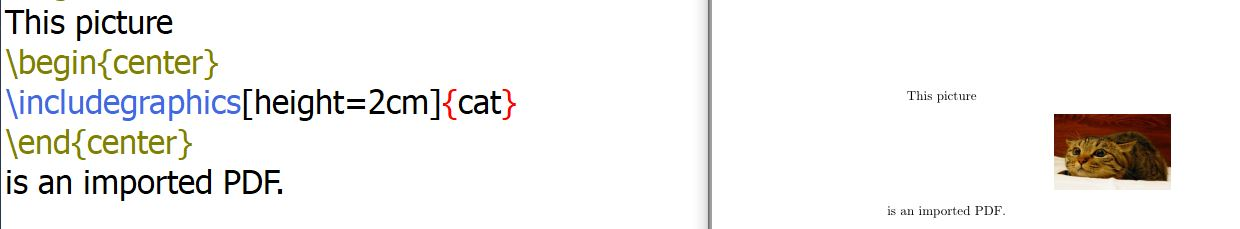
\includegraphics[width=0.5\textwidth]{1.JPG}
\caption{Вставка изображения}
\label{fig:insert_image}
\end{figure}

\subsection{Способы редактирования изображения}

Но работая с изображениями зачастую нам нужно изменять их форму или размер, для этого существуют различные функции.

\subsubsection{Увеличение ширины и высоты}

Данная функция достаточно понятна по принципу работы, но есть важный момент: когда вы будете увеличивать или уменьшать один из этих параметров вашего изображения, для того, чтобы избежать искажения исходного изображения, второй параметр будет подстраиваться программой автоматически.

\begin{figure}[h]
\centering
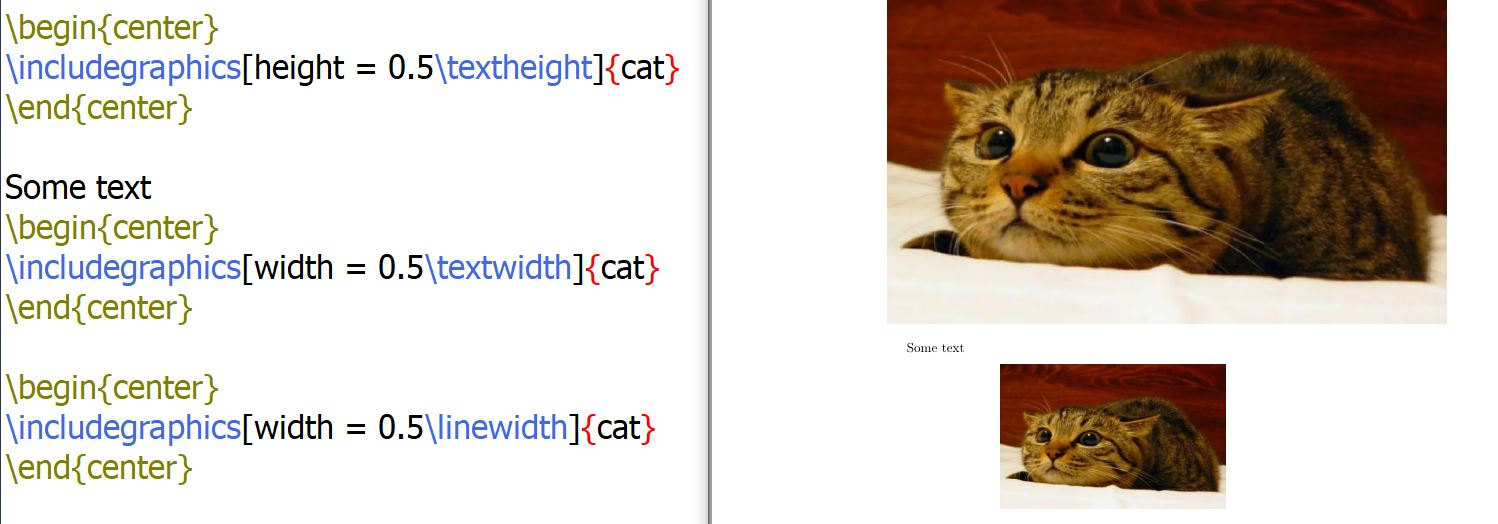
\includegraphics[width=0.5\textwidth]{2.JPG}
\caption{Изменение ширины и высоты изображения}
\label{fig:width_height}
\end{figure}

\subsubsection{Поворот и масштабирование изображения}

Для поворота изображения используется параметр \texttt{angle} со значением угла, на который вы хотите его повернуть.

Параметр \texttt{scale}, в свою очередь, используется для того, чтобы настроить масштаб исходного изображения.

\begin{figure}[h]
\centering
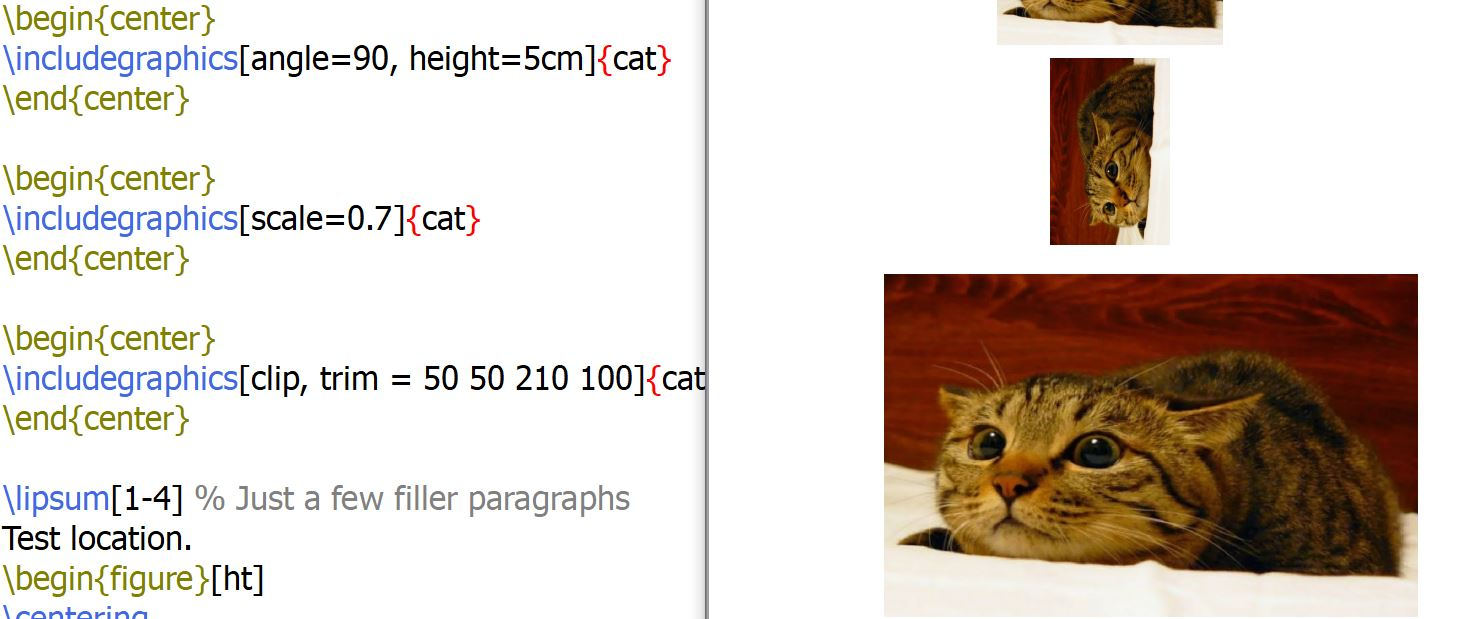
\includegraphics[width=0.5\textwidth]{3.JPG}
\caption{Поворот и масштабирование изображения}
\label{fig:rotate_scale}
\end{figure}

\subsubsection{Обрезка изображения}

Параметры \texttt{clip} и \texttt{trim} позволяют нам обрезать наше исходное изображение. В данной комбинации \texttt{clip}, имеющий по умолчанию значение true, обозначает отсечение части рисунка, а \texttt{trim} задает расстояния между левыми, нижними, правыми и верхними границами. Соответственно, изменяя эти параметры, мы можем получить ту часть изображения, которая нам нужна.

\begin{figure}[h]
\centering
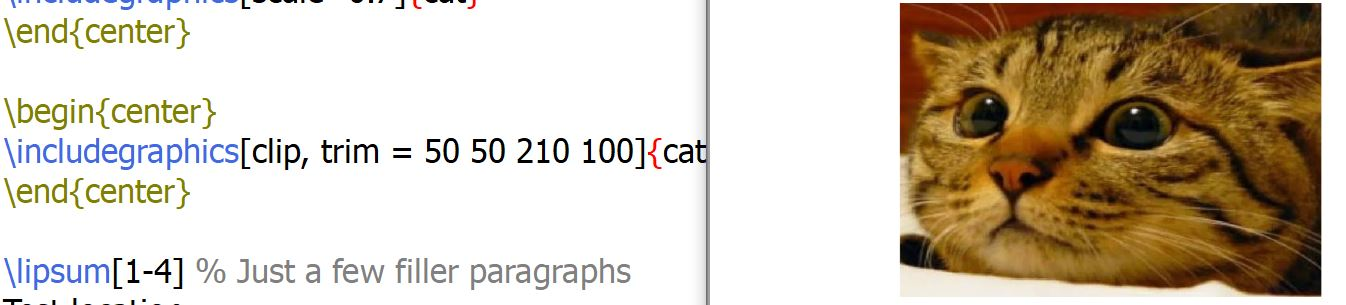
\includegraphics[width=0.5\textwidth]{4.JPG}
\caption{Обрезка изображения}
\label{fig:clip_trim}
\end{figure}

\subsection{Добавление изображения внутрь текста}

При добавлении изображения есть несколько параметров размещения, которые указаны ниже с их описанием, также их можно комбинировать, как показано на примере.

Важно, что в таком случае в \texttt{begin} и \texttt{end} мы должны указать \texttt{figure}.

При таком добавлении, как в предыдущей лабораторной работе, связанной с уравнениями, изображения будут нумероваться, что в дальнейшем дает возможность на них удобно ссылаться в документе. Нумерация происходит автоматически.

\begin{itemize}
\item \textbf{h} - «Здесь» (если возможно)
\item \textbf{b} - в верхней части страницы
\item \textbf{t} - в нижней части страницы
\item \textbf{p} - на специальной странице, предназначенной только для плавающих объектов
\end{itemize}

\begin{figure}[h]
\centering
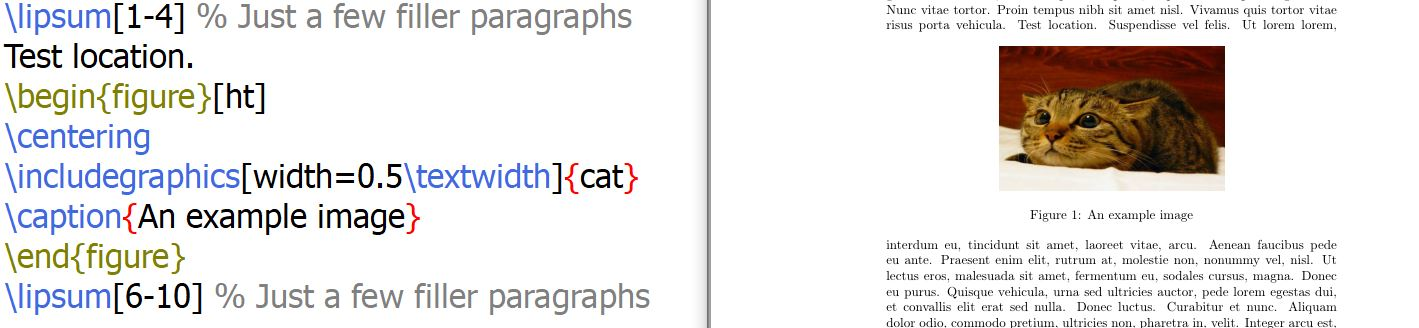
\includegraphics[width=0.5\textwidth]{5.JPG}
\caption{Размещение изображения в тексте}
\label{fig:placement}
\end{figure}

На втором примере параметр H - это строгий параметр, и зачастую лучше избегать его использования, так как это может плохо повлиять на структуру документа, например, останется много пустого места.

\begin{figure}[h]
\centering
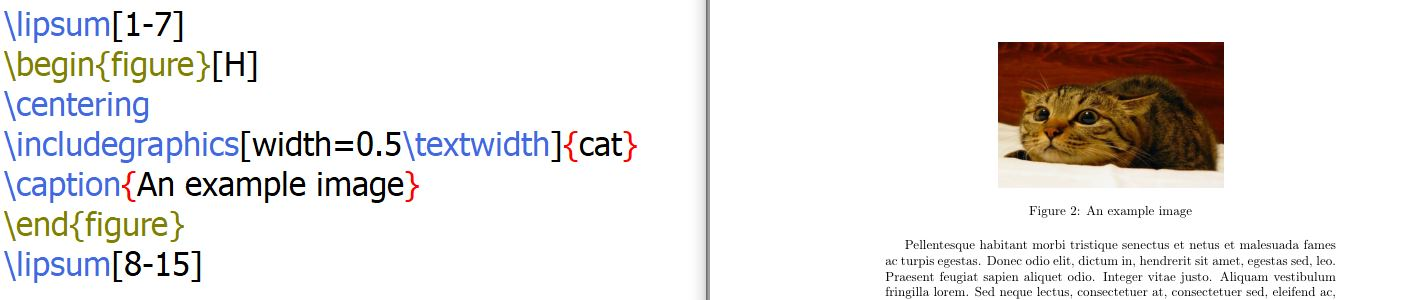
\includegraphics[width=0.5\textwidth]{6.JPG}
\caption{Использование строгого размещения H}
\label{fig:strict_placement}
\end{figure}

\subsection{Ссылки и гиперссылки}

Для того, чтобы создавать обычные ссылки в \LaTeX, существует встроенная функция. Объект для будущей ссылки необходимо отмечать, используя \texttt{label}, а для того, чтобы уже вставить эту ссылку, используется \texttt{ref}.

\begin{figure}[h]
\centering
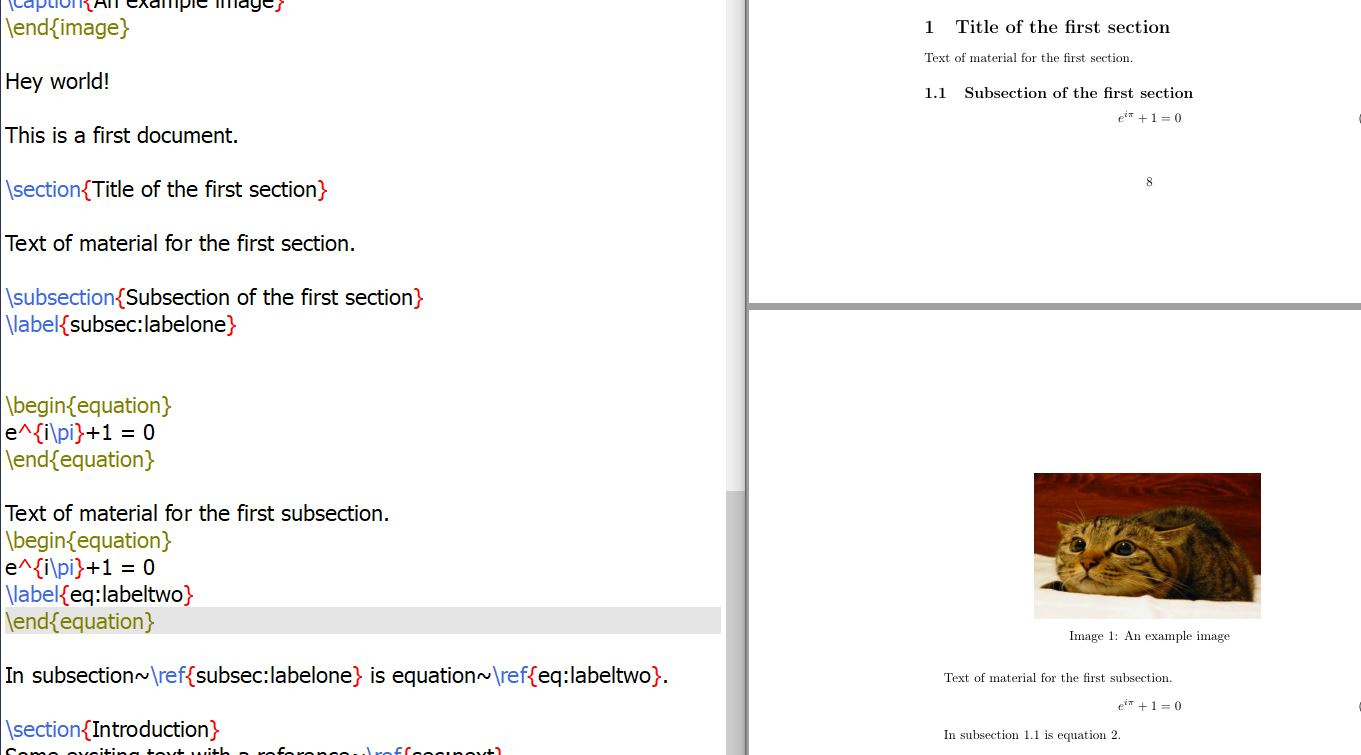
\includegraphics[width=0.5\textwidth]{7.JPG}
\caption{Создание ссылок}
\label{fig:references}
\end{figure}

Однако, если вы хотите вставить гиперссылку, которая при нажатии будет отправлять вас к выбранному элементу, то сам способ точно такой же, но необходимо добавить специальный пакет для гиперссылок, который был указан в самом начале.

\begin{figure}[h]
\centering
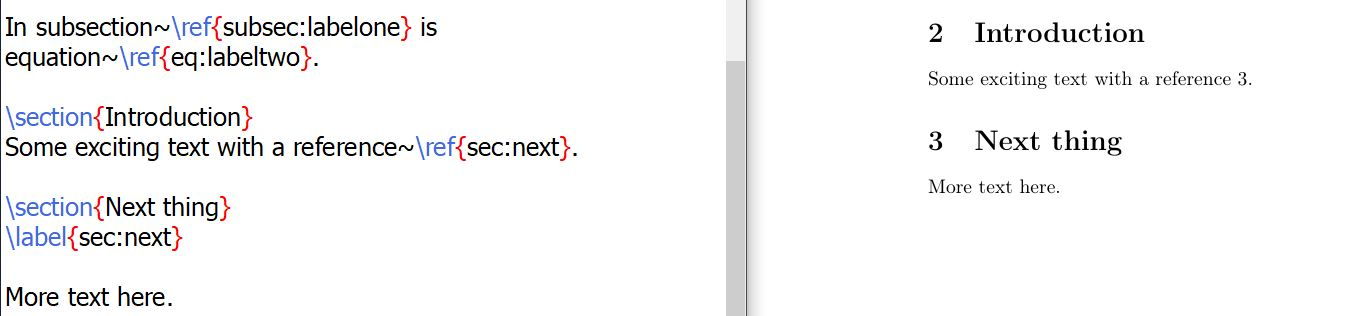
\includegraphics[width=0.5\textwidth]{8.JPG}
\caption{Создание гиперссылок}
\label{fig:hyperlinks}
\end{figure}

\section{Выводы}

В процессе выполнения данной лабораторной работы я научилась добавлять и редактировать графические изображения в среде \LaTeX, а также создавать ссылки и гиперссылки при работе с документом.

\begin{thebibliography}{9}
\bibitem{posobie} 
Пособие по лабораторным работам
\end{thebibliography}

\end{document}